\chapter{System Description} 

%Pg 66

\section{Configuration}
%Levitating one magnet - repulsive
%	Vs other configurations
%	

%TODO: introduction or change

The magnetic levitation system is considered in its SISO (single input, single output) system configuration as it levitates a magnet via repulsion.
%	Repulsive
As such, only the bottom coil and magnet are considered as shown in the simplified diagram \ref{fig:projSys}.

%INSERT DIAGRAM
\begin{figure}[h]
    \centering
    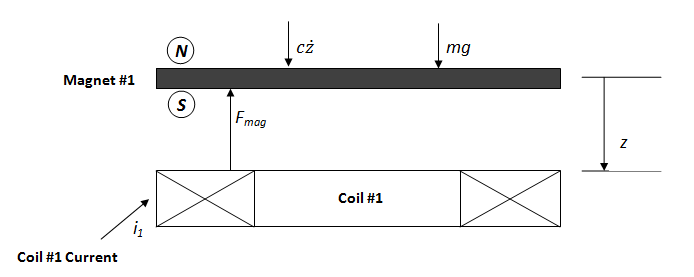
\includegraphics[width=.9\textwidth]{projSys}
    \caption{System Diagram}
    \label{fig:projSys}
\end{figure}

In this model, there are 3 forces acting on the magnet: the force of gravity ($mg$), the force of friction ($c\dot{z}$) and the magnetic force form the drive coil ($F_{mag}$).

\section{State Space Model - Inputs, Outputs and State Variables}

For the system modeling done in this report, y denotes the output variable, u denotes the input variable and the vector \textbf{x} denotes the state variables.
%SISO here 

\subsection{Inputs}
The input to the system is the current in Coil \#1, denoted in diagram \ref{fig:projSys} by $i_{1}$.
This is given in equation \ref{eq:input}.

\begin{equation}
	\label{eq:input}
	\textbf{u} = \left[\begin{array}{c}i_{1}\end{array}\right]
\end{equation}

\subsection{State Variables}
\label{sec:statevars}

The state variables for the system are chosen to be the the magnets velocity ($\dot{z}$) and its position ($z$). 
This is shown in equation \ref{eq:statevars}

\begin{equation}
	\label{eq:statevars}
	{\bf x} = 
	\left[
		\begin{array}{c}
			x_{1} \\
			x_{2} \\
		\end{array}
	\right]
	=
	\left[
		\begin{array}{c}
			z \\
			\dot{z} \\
		\end{array}
	\right]
\end{equation}

\subsection{Output}
The output of the system is the position of the disk magnet, denoted in diagram \ref{fig:projSys} by $z$.
This is shown in equation \ref{eq:output}:

\begin{equation}
	\label{eq:output}
	\textbf{y} = 
	\left[\begin{array}{c}z\end{array}\right] %= 
	%\left[\begin{array}{c}x_{1}\end{array}\right]
\end{equation}